% BehaVerify landing-page pipeline diagram.
% Build: pdflatex pipeline.tex
% Convert: dvisvgm --pdf pipeline.pdf -o ../img/pipeline.svg
% Committed output: ../img/pipeline.svg (vector) + ../img/pipeline.png (raster)
\documentclass[border=6pt,tikz]{standalone}
\usepackage{tikz}
\usepackage{amsmath, amssymb}
\usepackage[T1]{fontenc}
\usepackage{lmodern}
\usetikzlibrary{arrows.meta, positioning, fit, shapes.geometric, shapes.multipart, calc, decorations.pathreplacing, backgrounds}

\tikzset{
  % blocks
  input/.style   = {draw, rounded corners=2pt, fill=blue!8,   align=center,
                    font=\small, inner sep=5pt, minimum width=2.2cm, minimum height=0.9cm},
  stage/.style   = {draw, rounded corners=2pt, fill=purple!10, align=center,
                    font=\small, inner sep=5pt, minimum width=2.6cm, minimum height=0.9cm},
  backend/.style = {draw, rounded corners=2pt, fill=orange!15, align=center,
                    font=\small, inner sep=4pt, minimum width=2.0cm, minimum height=0.85cm},
  output/.style  = {draw, rounded corners=2pt, fill=green!12,  align=center,
                    font=\small, inner sep=4pt, minimum width=2.0cm, minimum height=0.85cm},
  verif/.style   = {draw, rounded corners=2pt, fill=red!10,    align=center,
                    font=\small, inner sep=4pt, minimum width=2.4cm, minimum height=0.95cm},
  future/.style  = {draw, rounded corners=2pt, fill=gray!10,  align=center, dashed,
                    font=\small\itshape, inner sep=4pt, minimum width=2.4cm, minimum height=0.95cm},
  group/.style   = {draw=black!40, rounded corners=6pt, inner sep=11pt,
                    fill=black!3, line width=0.6pt},
  grouplabel/.style = {font=\footnotesize\bfseries, text=black!70,
                       anchor=south, inner sep=0pt, outer sep=0pt},
  % arrows
  flow/.style = {-{Latex[length=2.6mm]}, line width=0.55pt, shorten >=1pt, shorten <=1pt},
  dashflow/.style = {-{Latex[length=2.6mm]}, dashed, line width=0.5pt, shorten >=1pt, shorten <=1pt},
}

\begin{document}
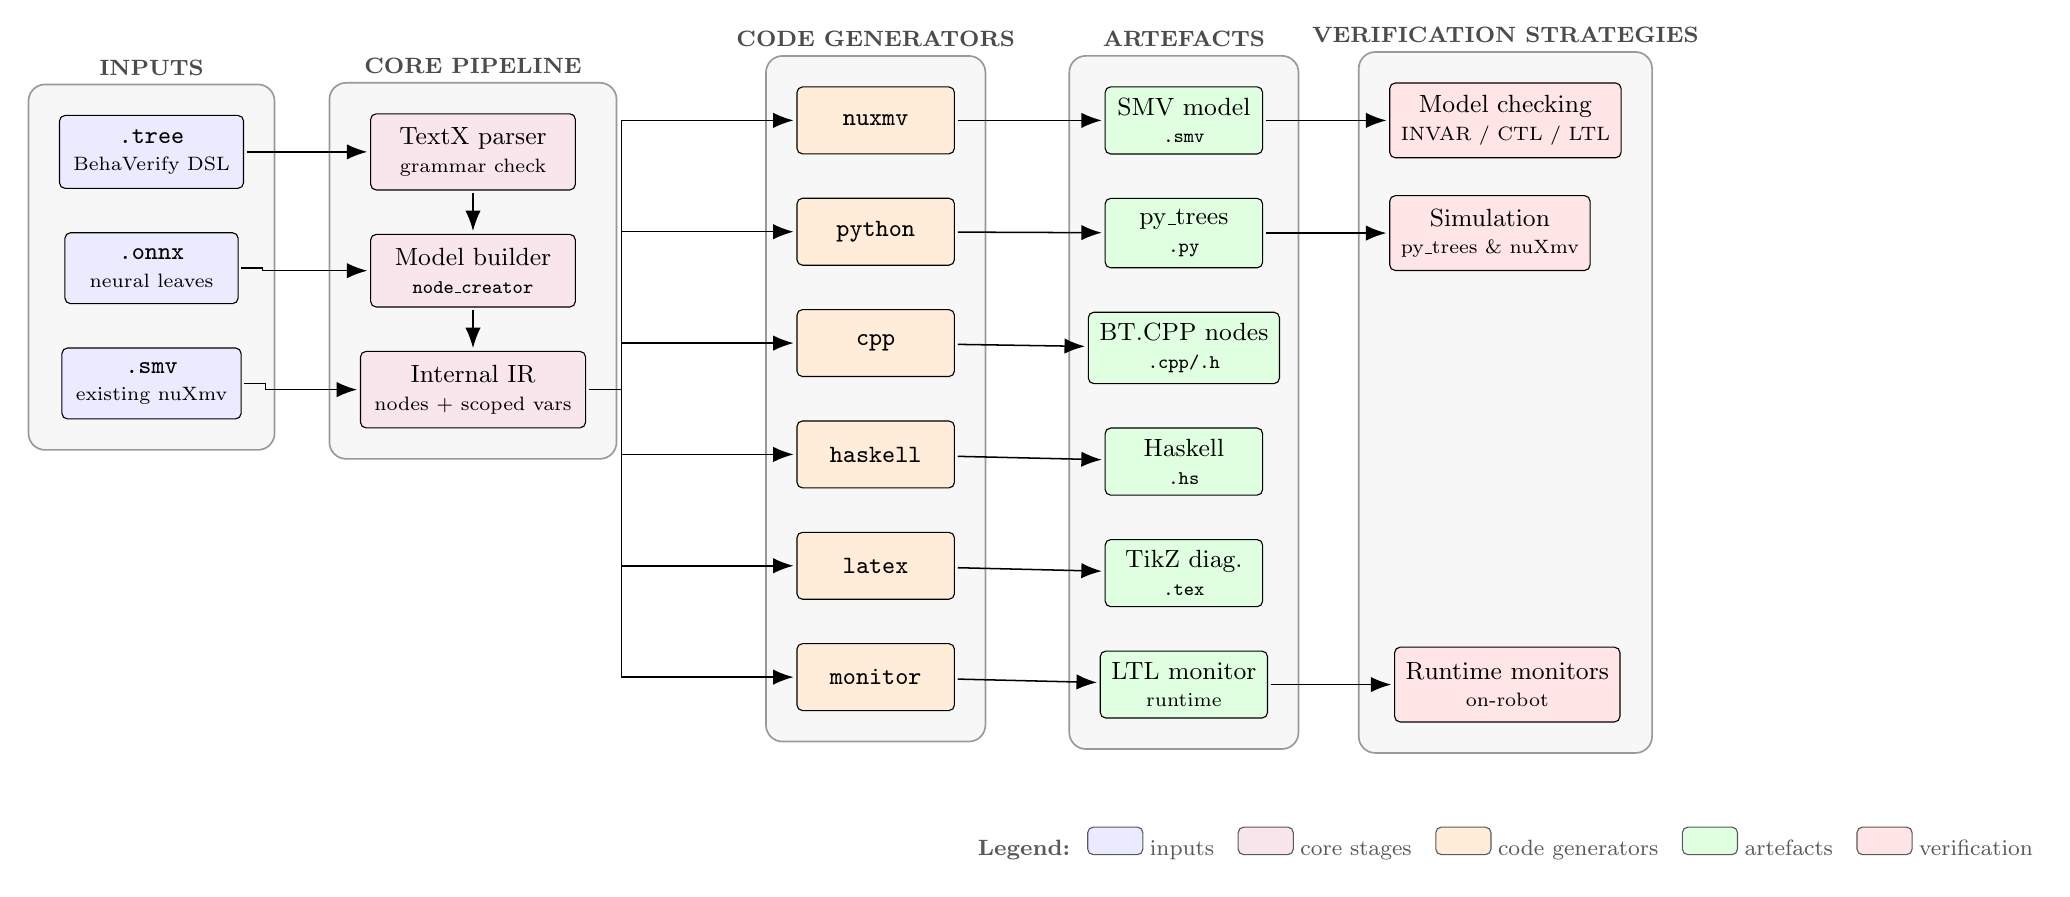
\begin{tikzpicture}[node distance=0.55cm and 0.85cm]

% ---------- Inputs ----------
\node[input] (tree) {\texttt{.tree}\\[-1pt]\scriptsize BehaVerify DSL};
\node[input, below=of tree] (onnx) {\texttt{.onnx}\\[-1pt]\scriptsize neural leaves};
\node[input, below=of onnx] (smv) {\texttt{.smv}\\[-1pt]\scriptsize existing nuXmv};

\begin{scope}[on background layer]
  \node[group, fit=(tree)(onnx)(smv)] (ginp) {};
\end{scope}
\node[grouplabel] at ([yshift=3pt]ginp.north) {INPUTS};

% ---------- Core ----------
\node[stage, right=1.6cm of tree] (parse)  {TextX parser\\[-1pt]\scriptsize grammar check};
\node[stage, below=of parse]      (model)  {Model builder\\[-1pt]\scriptsize \texttt{node\_creator}};
\node[stage, below=of model]      (ir)     {Internal IR\\[-1pt]\scriptsize nodes + scoped vars};

\begin{scope}[on background layer]
  \node[group, fit=(parse)(ir)] (gcore) {};
\end{scope}
\node[grouplabel] at ([yshift=3pt]gcore.north) {CORE PIPELINE};

% ---------- Backends ----------
\node[backend, right=2.8cm of parse.east,  yshift=0.4cm] (bnuxmv) {\texttt{nuxmv}};
\node[backend, below=of bnuxmv]                          (bpy)    {\texttt{python}};
\node[backend, below=of bpy]                             (bcpp)   {\texttt{cpp}};
\node[backend, below=of bcpp]                            (bhs)    {\texttt{haskell}};
\node[backend, below=of bhs]                             (blatex) {\texttt{latex}};
\node[backend, below=of blatex]                          (bmon)   {\texttt{monitor}};

\begin{scope}[on background layer]
  \node[group, fit=(bnuxmv)(bmon)] (gback) {};
\end{scope}
\node[grouplabel] at ([yshift=3pt]gback.north) {CODE GENERATORS};

% ---------- Outputs (artefacts) ----------
\node[output, right=1.9cm of bnuxmv] (onuxmv) {SMV model\\[-1pt]\scriptsize \texttt{.smv}};
\node[output, below=of onuxmv]       (opy)    {py\_trees\\[-1pt]\scriptsize \texttt{.py}};
\node[output, below=of opy]          (ocpp)   {BT.CPP nodes\\[-1pt]\scriptsize \texttt{.cpp/.h}};
\node[output, below=of ocpp]         (ohs)    {Haskell\\[-1pt]\scriptsize \texttt{.hs}};
\node[output, below=of ohs]          (olatex) {TikZ diag.\\[-1pt]\scriptsize \texttt{.tex}};
\node[output, below=of olatex]       (omon)   {LTL monitor\\[-1pt]\scriptsize runtime};

\begin{scope}[on background layer]
  \node[group, fit=(onuxmv)(omon)] (gout) {};
\end{scope}
\node[grouplabel] at ([yshift=3pt]gout.north) {ARTEFACTS};

% ---------- Verification strategies (right column, aligned with feeder artefact) ----------
\node[verif, right=1.6cm of onuxmv] (vmc)  {Model checking\\[-1pt]\scriptsize INVAR / CTL / LTL};
\node[verif, right=1.6cm of opy]    (vsim) {Simulation\\[-1pt]\scriptsize py\_trees \& nuXmv};
\node[verif, right=1.6cm of omon]   (vmon) {Runtime monitors\\[-1pt]\scriptsize on-robot};

% --- BEGIN reserved future block: uncomment to re-enable ---
% Place a dashed "Probabilistic (planned)" node below vmon, and add an
% additional dashed arrow from ir.east. Remember to add vsbt to the
% ``\node[group, fit=...]`` below so the group box grows to include it.
%
% \node[future, below=of vmon] (vsbt)
%   {Probabilistic\\[-1pt]\scriptsize stochastic BTs (planned)};
% \coordinate (irright) at ($(ir.east) + (0.4cm, 0)$);
% \draw[dashflow] (ir.east) -- (irright) |- (vsbt.west);
% --- END reserved future block ---

\begin{scope}[on background layer]
  \node[group, fit=(vmc)(vsim)(vmon)] (gver) {};
\end{scope}
\node[grouplabel] at ([yshift=3pt]gver.north) {VERIFICATION STRATEGIES};

% ---------- Flow: INPUTS -> CORE ----------
\draw[flow] (tree)  -- (parse);
\draw[flow] (onnx.east) -- ++(0.3cm,0) |- (model.west);
\draw[flow] (smv.east)  -- ++(0.3cm,0) |- (ir.west);

% ---------- Flow: CORE chain ----------
\draw[flow] (parse) -- (model);
\draw[flow] (model) -- (ir);

% ---------- Flow: IR -> backends ----------
\foreach \b in {bnuxmv, bpy, bcpp, bhs, blatex, bmon} {
  \draw[flow] (ir.east) -- ++(0.45cm,0) |- (\b.west);
}

% ---------- Flow: backends -> artefacts ----------
\draw[flow] (bnuxmv) -- (onuxmv);
\draw[flow] (bpy)    -- (opy);
\draw[flow] (bcpp)   -- (ocpp);
\draw[flow] (bhs)    -- (ohs);
\draw[flow] (blatex) -- (olatex);
\draw[flow] (bmon)   -- (omon);

% ---------- Flow: artefacts -> verification strategies (direct, same-row) ----------
\draw[flow] (onuxmv) -- (vmc);
\draw[flow] (opy)    -- (vsim);
\draw[flow] (omon)   -- (vmon);

% ---------- Legend ----------
\node[below=0.8cm of gver.south, align=center, font=\footnotesize, text=black!65]
  (legend)
  {\textbf{Legend:}\;
   \tikz\node[input,minimum width=0.7cm,minimum height=0.35cm,inner sep=0pt]{};\;inputs\quad
   \tikz\node[stage,minimum width=0.7cm,minimum height=0.35cm,inner sep=0pt]{};\;core stages\quad
   \tikz\node[backend,minimum width=0.7cm,minimum height=0.35cm,inner sep=0pt]{};\;code generators\quad
   \tikz\node[output,minimum width=0.7cm,minimum height=0.35cm,inner sep=0pt]{};\;artefacts\quad
   \tikz\node[verif,minimum width=0.7cm,minimum height=0.35cm,inner sep=0pt]{};\;verification};
   % --- Legend entry reserved for the future "planned" block; uncomment to re-enable ---
   % \quad \tikz\node[future,minimum width=0.7cm,minimum height=0.35cm,inner sep=0pt]{};\;planned

\end{tikzpicture}
\end{document}
